\documentclass{standalone}
\usepackage{tikz}

\usetikzlibrary{matrix,positioning,shapes.arrows,fit}

\tikzset{ 
table/.style={
  matrix of nodes,
  row sep=-\pgflinewidth,
  column sep=-\pgflinewidth,
  nodes={
    rectangle,draw,
    text width=0.5cm,
    %minimum width=0.75cm,
    %minimum height=0.75cm,
    align=center},
  text depth=0.125cm,
  text height=0.25cm,
  nodes in empty cells
  },
%texto/.style={font=\footnotesize\sffamily},
%title/.style={font=\small\sffamily}
}

\begin{document}
    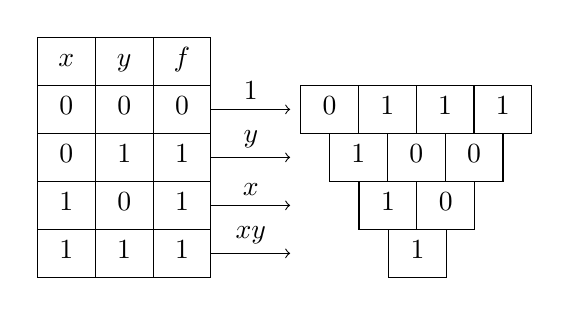
\begin{tikzpicture}
        \matrix [table] (f)
        {
             $x$ & $y$ & $f$ \\ 
             0 & 0 & 0 \\
             0 & 1 & 1 \\
             1 & 0 & 1 \\
             1 & 1 & 1 \\
        };
        \matrix [table, right=of f-2-3.east] (r0)
        {
            0 & 1 & 1 & 1 \\
        };
        \matrix [table,
            right=of f-3-3.east, 
            outer sep=0.375cm
            ] 
            (r1)
        {
            1 & 0 & 0 \\
        };\matrix [table, right=of f-4-3.east, outer sep=0.75cm] (r2)
        {
            1 & 0 \\
        };
        \matrix [table, right=of f-5-3.east, outer sep=1.125cm] (r3)
        {
            1 \\
        };
        \draw [->] (f-2-3.east) -- node [above] {1} (r0.west);
        \draw [->] (f-3-3.east) -- node [above] {$y$} (r1.west);
        \draw [->] (f-4-3.east) -- node [above] {$x$} (r2.west);
        \draw [->] (f-5-3.east) -- node [above] {$xy$} (r3.west);
    \end{tikzpicture}
\end{document}